\begin{pastexam}[label={px:gk3-098-ds-04}]{高考三級資訊處理 98 年 第四題}
（申論；26 分）

假設有一個 C 語言函式如下（左側數字為列號，非程式之一部分）：
\begin{minted}[fontsize=\small, style=perldoc, linenos, xleftmargin=2.5em]{c}
int f(int n)
{
if (n == 0)
      return(0);
if (n == 1)
    return(1);
printf("ADD ");
return (f (n-1) + f (n-2));
}
\end{minted}
\begin{itemize}[leftmargin=2.2em]
\item[㈠] 以 f(4)呼叫上面函式，會列印出多少個"ADD"？（6 分）
\item[㈡] 如果以 f(n)呼叫上面函式，n 為任意正整數，程式執行完畢後，會列印出多少個"ADD"？請推導其通式
（只要推導出其關係式即可）。（12 分）
\item[㈢] 在忽略第 7 列的情形下，可將上面函式改寫成更有效率的函式如下。請完成第 10\textasciitilde 12 列
的程式內容。（8 分）
\end{itemize}
\begin{minted}[fontsize=\small, style=perldoc, linenos, xleftmargin=2.5em]{c}
int f(int n)
{
int i, a,b,c;
if (n <= 1)
    return(n);
a=0;
b=1;
for (i = 2; i <= n; i++)
{



} // end of for
return (c);
}
\end{minted}
\end{pastexam}

\begin{pastsoln}
答案：㈠ $4$ 個；㈡ $A(n) = A(n-1) + A(n-2) + 1$，$A(0) = A(1) = 0$，解出來 $A(n) = F_{n+1} - 1$
（$F$ 是費氏數列）；㈢ 第 10--12 列是 \texttt{c = a + b;}、\texttt{a = b;}、\texttt{b = c;}。

這個函式算的是費氏數 $F_n$（$F_0 = 0$、$F_1 = 1$、$F_n = F_{n-1} + F_{n-2}$）。 第 7 列在 $n \ge 2$
時才會執行，每次這樣的呼叫印一個 \texttt{ADD}，所以「印幾個 ADD」等於「遞迴樹裡有幾個 $n \ge 2$ 的
呼叫」。

\textbf{㈠} 畫出 \texttt{f(4)} 的遞迴樹，$n \ge 2$ 的節點加框（每個印一次 ADD）：
\begin{center}
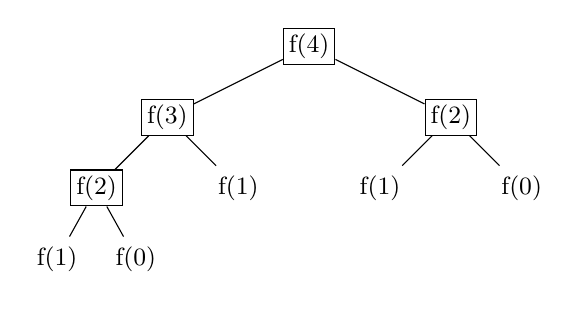
\begin{tikzpicture}[v/.style={draw=none,font=\small},a/.style={draw,rectangle,font=\small,inner sep=2pt},
    level distance=9mm, level 1/.style={sibling distance=36mm},
    level 2/.style={sibling distance=18mm}, level 3/.style={sibling distance=10mm}]
\node[a] {f(4)}
  child {node[a] {f(3)}
    child {node[a] {f(2)} child {node[v] {f(1)}} child {node[v] {f(0)}}}
    child {node[v] {f(1)}}}
  child {node[a] {f(2)}
    child {node[v] {f(1)}}
    child {node[v] {f(0)}}};
\end{tikzpicture}
\end{center}
加框的是 f(4)、f(3)、f(2)、f(2)，共 $\mathbf{4}$ 個 ADD。

\textbf{㈡} 令 $A(n)$ 是呼叫 \texttt{f(n)} 印出的 ADD 個數。 $n = 0$、$1$ 時直接 return，
$A(0) = A(1) = 0$。 $n \ge 2$ 時自己印一個，再加上兩個遞迴呼叫印的：
\[
A(n) = A(n-1) + A(n-2) + 1, \qquad n \ge 2.
\]
逐項算：$A(2) = 1$、$A(3) = 2$、$A(4) = 4$、$A(5) = 7$、$A(6) = 12$、$A(7) = 20$。 這和費氏數
$F_3, F_4, \ldots = 2, 3, 5, 8, 13, 21$ 都差 $1$。 證明：令 $B(n) = A(n) + 1$，代入得
\[
B(n) = (A(n-1) + 1) + (A(n-2) + 1) = B(n-1) + B(n-2),\qquad B(0) = B(1) = 1,
\]
和 $F_{n+1}$ 的遞迴式、初始值（$F_1 = F_2 = 1$）都一樣，所以 $B(n) = F_{n+1}$，
\[
A(n) = F_{n+1} - 1 = \frac{1}{\sqrt5}\left(\Bigl(\frac{1+\sqrt5}{2}\Bigr)^{n+1}
- \Bigl(\frac{1-\sqrt5}{2}\Bigr)^{n+1}\right) - 1.
\]
（費氏數的封閉形式見資結書第~2.5~節的線性遞迴。）檢查：$A(4) = F_5 - 1 = 5 - 1 = 4$，和㈠一樣。 ADD 個數隨 $n$
指數成長（約 $1.618^n$），這就是遞迴版沒有效率的原因：同一個 \texttt{f(k)} 被重算很多次。

\textbf{㈢} 由下往上算，只留最後兩項：進入第 $i$ 輪時 $a = F_{i-2}$、$b = F_{i-1}$。
\begin{minted}[fontsize=\small, style=perldoc, linenos, firstnumber=10, xleftmargin=2.5em]{c}
c = a + b;   /* c = F(i) */
a = b;       /* 下一輪的 F(i-1) */
b = c;       /* 下一輪的 F(i) */
\end{minted}
迴圈不變量：第 $i$ 輪開始時 $a = F_{i-2}$、$b = F_{i-1}$。 $i = 2$ 時 $a = 0 = F_0$、$b = 1 = F_1$ 成立；
這一輪算出 $c = F_i$，再把 $a, b$ 往前移成 $F_{i-1}, F_i$，下一輪仍成立。 迴圈最後一輪 $i = n$，
$c = F_n$，第 14 列回傳正確。 $n \ge 2$ 才會進迴圈，所以 $c$ 一定有值；$n \le 1$ 由第 4--5 列處理。
時間從指數降到 $O(n)$，空間 $O(1)$。 這是動態規劃「由下往上、只留需要的幾格」的寫法（資結書第~18.1~節）。
例：$n = 4$ 時三輪的 $(c, a, b)$ 依序是 $(1, 1, 1)$、$(2, 1, 2)$、$(3, 2, 3)$，回傳 $3 = F_4$。
\end{pastsoln}
